\documentclass[11pt]{article}
\usepackage{fullpage}
\usepackage{epsfig}
\usepackage{algorithm}
\usepackage[noend]{algorithmic}
\usepackage{amsmath,amssymb,amsthm}
\usepackage{enumerate}
\usepackage{framed}
\usepackage{titlesec}
\usepackage{listings}
\usepackage{tabto}
\usepackage{xcolor}
\usepackage{hyperref}

\usepackage{graphicx}
\usepackage{caption}
\usepackage{subcaption}

\usepackage{enumitem}

% FILL IN THE SPECIFICS OF EACH HOMEWORK HERE
\newcommand{\course}{EECS 446}
\newcommand{\semester}{Spring 2020}
\newcommand{\name}{Kernel and Other Low-level Software Development}
%%%
%%%
%%% PLEASE FILL OUT YOUR NAME AND THE HOMEWORK/PROBLEM NUMBER
%%% DO NOT INCLUDE STUDENT NAMES, FOR ANONYMOUS PEER GRADING PURPOSES.
%%%
%%%
\newcommand{\hwk}{Final Report}

\newcommand{\reportname}{ATA Driver Report}


\usepackage[margin=3cm]{caption}


%%% You can ignore the following stuff, it's just for formatting purposes
\textheight=8.6in
\setlength{\textwidth}{6.44in}
\addtolength{\headheight}{\baselineskip}
% enumerate uses a), b), c), ...
\renewcommand{\labelenumi}{\alph{enumi})}
% Sets the style for fancy pages (namely, all but first page)
% Changes the title box on the first page
\renewcommand\maketitle{
\begin{center}
  {\huge\bf\reportname}\\
\begin{tabular*}{6.44in}{l @{\extracolsep{\fill}}c r}
%\bfseries  &  & \bfseries \course ~\semester \\
%\bfseries&  & \bfseries  \hwk  \\
\bfseries   &   &  \bfseries \\
\bfseries   &   &  \bfseries \\
Name: Ashwin Chidambaram, SID:\bfseries  &  & \bfseries \course ~\semester\\
\-\hspace{1.15cm} Ujjwal Sai, SID: \bfseries&  & \bfseries  \hwk \\
\-\hspace{1.15cm} Haoxuan Zhang, SID: 3173595
\end{tabular*}
\end{center} }


%% adjustments for dynamic programming.

%\titleformat{\subsection}{\bf}{Part \thesubsection:}{1ex}{}
\titleformat{\section}[runin]{\normalsize\bfseries}{\thesection.}{5pt}{}
%\renewcommand{\thesubsection}{\alph{subsection}}
\titleformat{\subsection}[runin]{\normalsize\bfseries}{\-\hspace{0.5cm}\thesubsection}{5pt}{}
%\titleformat{\section}{\wrap}{}{}{}{}



%%
%%
%% THE REAL STUFF STARTS HERE
%%
%%
\begin{document}
\maketitle
\titlelabel{\thetitle.\quad}

\section{Section 1 \\}
Text Example \\
A new line!\\

A new line!

\subsection{subsection 1 \\}
Test Example \\
A new line!\\

A new line!\\
\-\hspace{1cm} indent 1 cm

%example for figure
\begin{figure}[h!]
  \center
  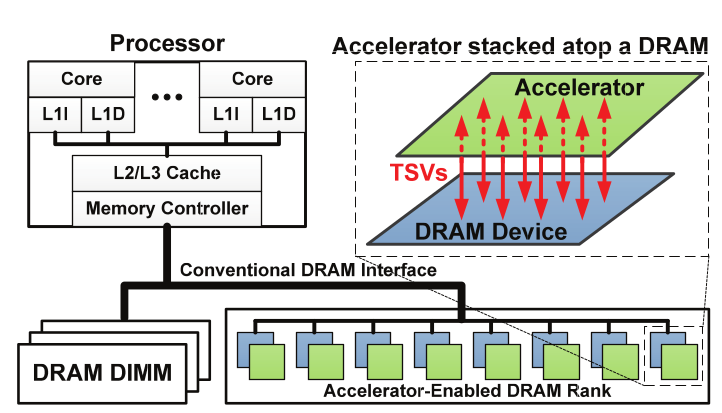
\includegraphics[width=0.5\textwidth]{./Figure/NDA.png}
  \caption{This is caption}
  \label{any_name}
\end{figure}

Reference Firgure \ref{any_name}

Reference 1: \cite{Ref1}
\section{Background\\\\}

\section{ATA DMA\\\\}

\section{ATA Interrupt\\\\}


\section{PCI support\\\\}

Our previous work for DMA and interrupt handling are only supporting legacy mode in which at most 4 drives could be detected at a well known location. The code of DMA and interrupt handling driver only supporting legacy mode is in the branch of \texttt{ata\_interrupts} in our Github repository. In our another branch \texttt{ATA\_PCI}, we tried to impliment PCI support with DMA and polling and it works correctly with legacy device testing. Because we didn't find a way to attach arbitrary number of IDE controllers to PCI bus, the driver is not tested with ata device located not in legacy location. This section, we will interpret the PCI mechnism and our work on PCI support for the ata driver.

\subsection{PCI Configuration Space\\\\}

Figure \ref{fig:cfg} shows the content of PCI configuration space.

\begin{figure}[h!]
  \center
  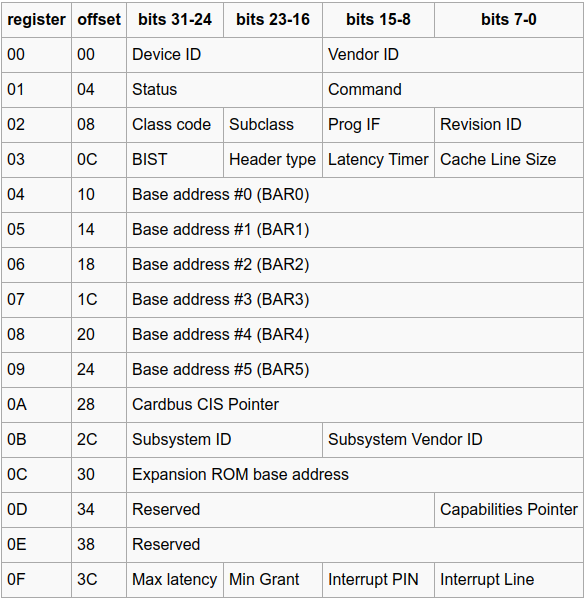
\includegraphics[width=0.5\textwidth]{./Figure/cfg.png}
  \caption{PCI Configuration Space\cite{OSDev_PCI}}
  \label{fig:cfg}
\end{figure}

The PCI configuration space has the I/O port mapped address at a well known places. It contains basic information of the device and the base address register which will be used to configure the base address of the device port registers.\\

According to OSdev PCI page\cite{OSDev_PCI}, the Class Code shown in Figure \ref{fig:cfg} contains class code, sub class code and program interface information which we would use to identify whether the device is an IDE device or not. The next subsection will illustrate the PCI native mode and how we obtain the base address of the device registers.


\subsection{PCI native mode\\\\}

Each ATA channel will have 8 I/O registers and 3 Control registers. The first step to utilize these registers is to find the location of the registers. Table \ref{tab:regs} shows the I/O port register address offset relative to the base address and the information is referenced from OSdev ATA PIO page\cite{OSDev_PIO}.\\

 \begin{table}[h!]
 \center
   \resizebox{0.5\textwidth}{!}{\begin{tabular}{| c | c |}
   \hline 
   Offset from I/O base(Direction) & Register \\
   \hline
   0 & Data register\\
   \hline
   1(Read) & Error Register\\
   \hline
   1(Write) & Feature Register\\
   \hline
   2 & Sector Count Register\\
   \hline
   3 & LAB low \\
   \hline
   4 & LBA mid \\
   \hline
   5 & LBA high \\
   \hline
   6 & Head register \\
   \hline
   7 (Read) & Status Register\\
   \hline
   7 (Write) & Command Register\\
   \hline
    \end{tabular}}
 \caption{ATA I/O registers}
 \label{tab:regs}
   
 \end{table}

ATA device also has 3 control register including Alternate Status Register, Device Control Register and Drive Address Register. We didn't use these registers in our driver except reading Alternate Status Register for delay.\\


Unlike the legacy mode where all the registers will be located at fixed and well known places, base addresses will be determined by Base Address Register. According to IDE controller programmer mannel\cite{IDE}, in primary channel, The I/O port base will be determined by BAR0, and the control port base will be determined by BAR1. In secondary channel, I/O port base will be determined by BAR2 while the control port base will be determined by BAR3.\\

To support DMA, we also need to get control of the bus master. The base address of the bus master is the value in BAR4 or BAR4 + 8 for primary channel or secondary channel. After obtaining the base address, we could use the address to access the I/O port mapped registers in the IDE controller including the ata drive registers and the bus master registers.\\

\subsection{Process of recognizing Device and Our Work on PCI}

To recognize the device, we would:
\begin{enumerate}
    \item Loop through PCI bus and devices to find devices having class code and subclass code to be 0x1 which means IDE device
    
    \item Allocate space for the IDE controller which contains 4 drive status
    \item Initialize members in drive status structure according to the channel, device ID and Base Address Register.
    \item Write to PCI configuration space command with 0x04 to enable Bus master
    \item Device detection and identification for each drive in the controller in the same way as the previous APIO ata driver.

\end{enumerate}

After detection and initializing the address information in the status structure, we would be able to utilize the information collected by the status structure to conduct read and write.\\

Our work on PCI is in the ATA\_PCI branch ata\_pci.c and the description of our works is as follows: 

\begin{enumerate}
    \item We could scan the PCI devices and register the device with name of ata(bus number)-(device number)-(channel)-(id)
    \item We initialize register addresses according to the base address registers.
    \item Because legacy mode ata devices are still attached to PCI bus, we tested our PCI support with legacy location and the testing result is still correct.
    \item We haven’t confirmed a way to add IDE controller attached with drives to the PCI bus so that we could test the driver with arbitrary device addresses.
\end{enumerate}

\section{Result}

\newpage
\begin{thebibliography}{9}
\bibitem{Ref1}
Reference Here

\bibitem{IDE}
Intel IDE Controller Programmer’s Reference Manual, November 2001, Revision 1.0

\bibitem{OSDev_PIO}
OSDev, ATA PIO Mode,
\url{https://wiki.osdev.org/ATA_PIO_Mode}, Retrieved on June 10

\bibitem{OSDev_PCI}
OSDev, PCI
\url{https://wiki.osdev.org/PCI}, Retrieved on June 10
\end{thebibliography}
\end{document}
